\documentclass{article}

\usepackage{amsmath}
\usepackage{mathtools}
\usepackage{amsfonts}
\usepackage{url}
\usepackage{xspace}
\usepackage{siunitx}
\usepackage{cancel}
\usepackage[usenames,dvipsnames]{xcolor}
\usepackage{tikz}
\usepackage{float}
\usepackage{booktabs}

% \usepackage{vletters}

% Formatting options 
\frenchspacing
% \setlength{\parindent}{0 ex}
% \setlength{\parskip}{3 ex plus 2 ex minus 1 ex}

% Defined macros

\DeclareMathOperator{\csch}{csch}
\DeclareMathOperator{\sech}{sech}

\newcommand{\degree}[0]{\ensuremath{^\circ}\xspace}
\renewcommand{\implies}{\Rightarrow}
\newcommand{\eval}[1]{\ensuremath{\left<#1\right>}}
\newcommand{\ket}[1]{\ensuremath{\left| #1 \right>}}
\newcommand{\bra}[1]{\ensuremath{\left< #1 \right|}}
\newcommand{\mel}[3]{\ensuremath{\left<#1 \right|\! #2 \!\left| #3 \right>}}
\newcommand{\proj}[2]{\ensuremath{\left<#1 \middle| #2 \right>}}

\newcommand{\pmat}[1]{\ensuremath{\begin{pmatrix}#1\end{pmatrix}}}

\newcommand{\pder}[2]{\ensuremath{\frac{\partial #1}{\partial #2}}}
\newcommand{\ppder}[2]{\ensuremath{\frac{\partial^2 #1}{\partial #2^2}}}
\newcommand{\ppmder}[3]{\ensuremath{\frac{\partial^2 #1}{\partial #2 \partial #3}}}

\newcommand{\pderc}[3]{\ensuremath{\left( \frac{\partial #1}{\partial #2} \right)_{\!\!#3}}}
\newcommand{\ppmderc}[4]{\ensuremath{\left( \frac{\partial^2 #1}{\partial #2 \partial #3} \right)_{\!\!#4}}}

\newcommand{\nuc}[2]{${}^{#1}\text{#2}$}

\newcommand{\fresco}[0]{\textsc{Fresco}\xspace}

% Titles and headers

\title{Phy 982 Homework 2}
\author{Josh Bradt and Chris Izzo}
\date{April 9, 2015}

\makeatletter
\let\thetitle\@title
\let\theauthor\@author
\makeatother

\usepackage{fancyhdr}
\pagestyle{fancy}
\chead{\footnotesize \MakeUppercase{\thetitle}} \rhead{\footnotesize\thepage}
\cfoot{}
\renewcommand{\headrulewidth}{0pt}

\begin{document}

\maketitle

\section*{Part I}

	We chose to use the nucleus \nuc{100}{Mo} for our target. This nucleus has 42 protons and 58 neutrons. As an even-even nucleus, this target has a ground state of $0^+$.

	We began by running \fresco for elastic scattering of protons at \SI{5}{MeV} and \SI{50}{MeV}. We did this for a point-like potential with a Coulomb radius of \SI{0.001}{fm} and a finite potential with a Coulomb radius of \SI{1.220}{fm}. We chose the second value from the previous homework assignment. Fig.~\ref{fig:protons_nonuc} shows the differential cross sections of these reactions as a ratio to the Rutherford cross sections. We can see that the ratio to Rutherford is approximately 1.0 for all angles for the scattering off of the point-like potential. This is because a point-like potential produces pure Coulomb scattering. For the finite-radius potentials, we found that the ratio to Rutherford is still 1.0 for the low-energy scattering. This is because the low-energy proton does not penetrate beyond the Coulomb radius. The higher-energy proton, on the other hand, penetrates beyond the Coulomb radius and sees that the potential is different from charge concentrated at a point. This explains why the \SI{50}{MeV} proton scattering off of the finite potential produces a cross section that is different from Rutherford, while the others do not.

	Next, we repeated this analysis with neutrons instead of protons. This gave us the elastic scattering cross sections shown in Fig.~\ref{fig:neutrons_nonuc}. As we can see, the scattering cross section is very small. This is because the neutrons are neutral and shouldn't interact with the Coulomb potential. 

	\begin{figure}
		\centering
		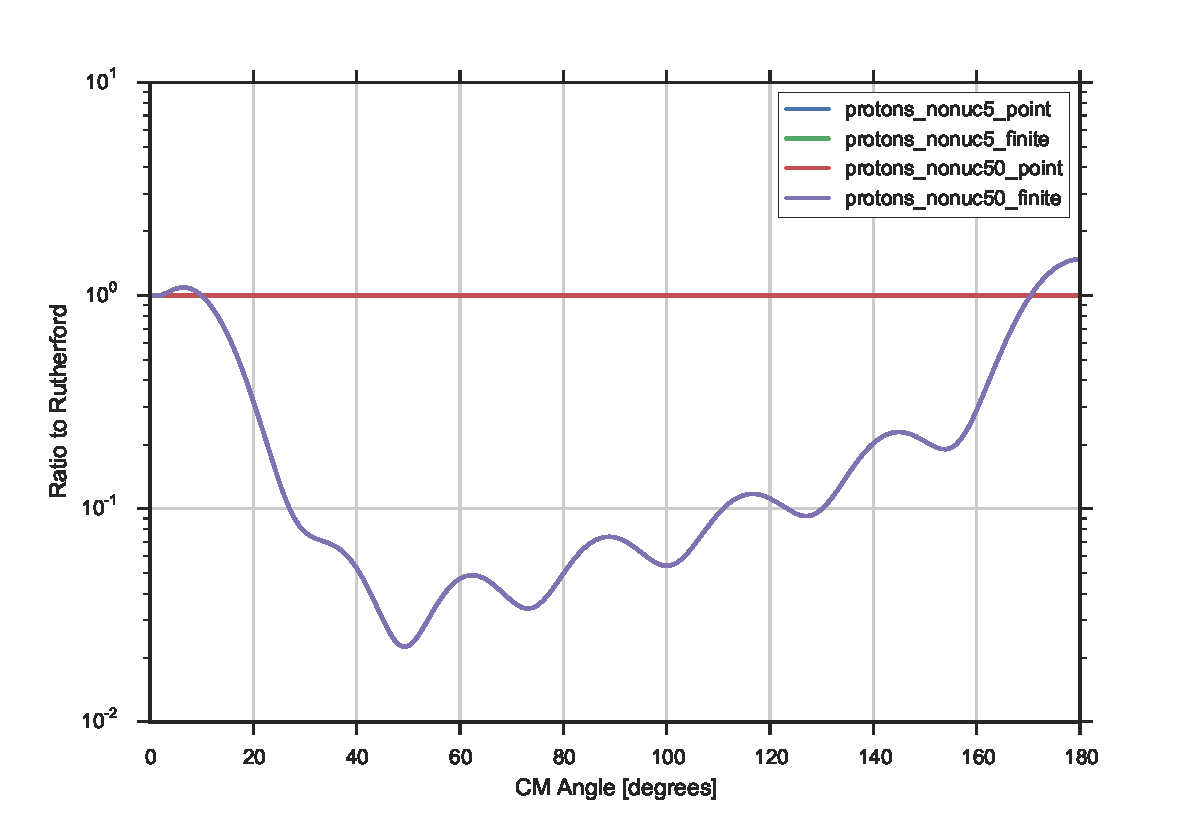
\includegraphics[width=\textwidth]{{images/protons_nonuc.pdf}}
		\caption{Elastic scattering cross sections for protons on \nuc{100}{Mo} at \SI{5}{MeV} and \SI{50}{MeV} for point-like and finite-radius potentials. This does not include a nuclear potential.}
		\label{fig:protons_nonuc}
	\end{figure}

	\begin{figure}
		\centering
		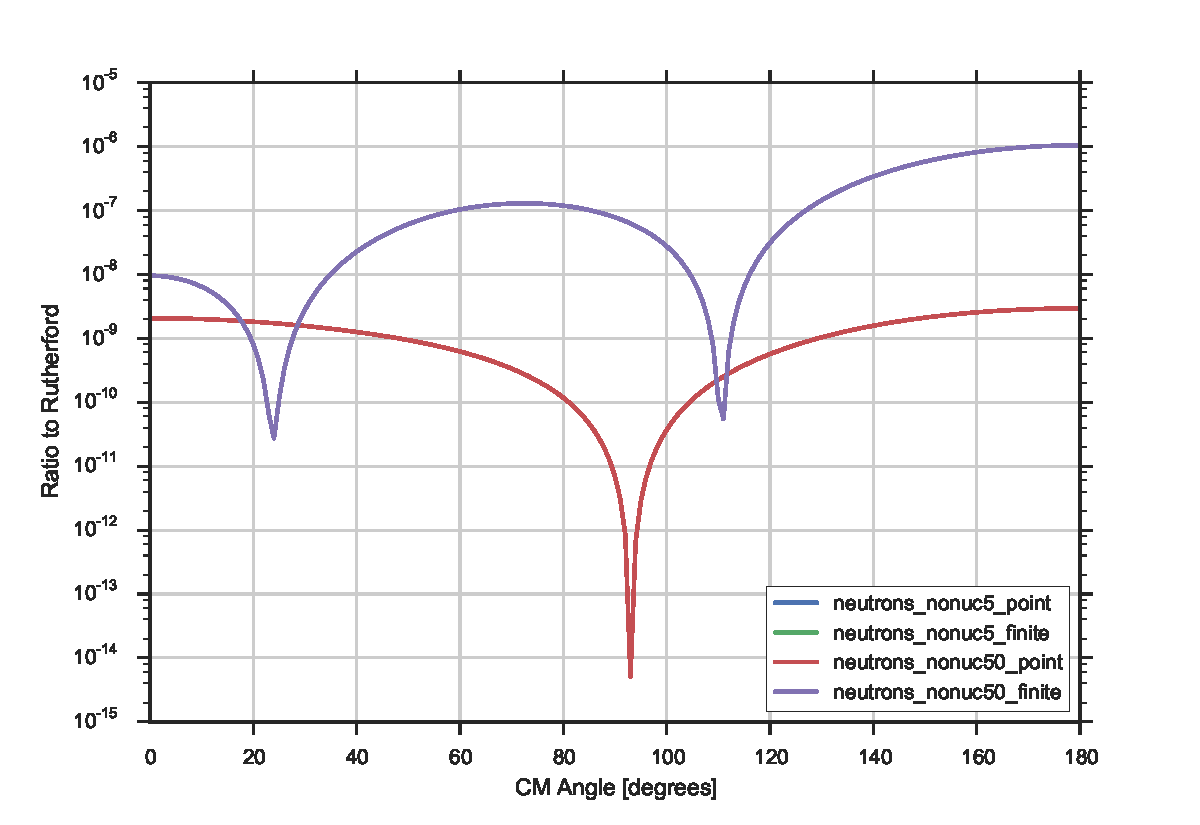
\includegraphics[width=\textwidth]{{images/neutrons_nonuc.pdf}}
		\caption{Elastic scattering cross sections for neutrons on \nuc{100}{Mo} at \SI{5}{MeV} and \SI{50}{MeV} for point-like and finite-radius potentials. This does not include a nuclear potential.}
		\label{fig:neutrons_nonuc}
	\end{figure}

	Next, we added a nuclear potential. We used a global optical potential of Woods-Saxon shape with parameters from Koning and Delaroche. \cite{Koning2003} We did this for both neutrons and protons. The angular distributions are shown in Fig.~\ref{fig:nuc_all}.

	We can see the following things:
	\begin{enumerate}
		\item For protons at low energy, the scattering cross sections are very close to Rutherford. This is because the low-energy proton does not probe beyond the Coulomb barrier.

		\item As before, the high-energy protons penetrate the Coulomb barrier. This leads to a more complex angular distribution since the proton sees the internal structure of the nucleus.

		\item For both energies, the neutrons probe the nuclear potential. This is because they are not affected by Coulomb repulsion. We also see that there is less scattering to backwards angles for the higher-energy neutrons.
	\end{enumerate}

	\begin{figure}
		\centering
		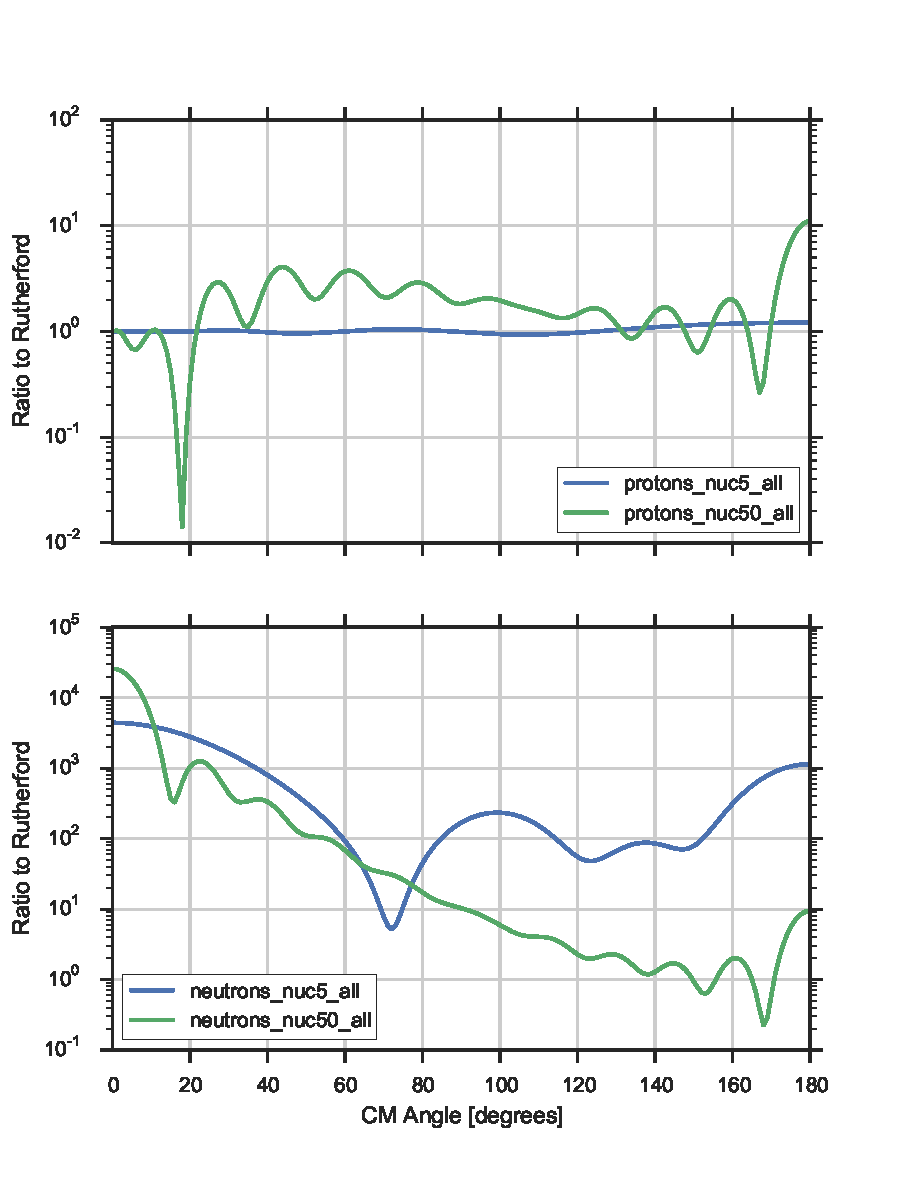
\includegraphics[width=\textwidth]{{images/nuc_all.pdf}}
		\caption{Elastic scattering cross sections on \nuc{100}{Mo} with a volume nuclear potential for protons (top) and neutrons (bottom) at \SI{5}{MeV} and \SI{50}{MeV}.}
		\label{fig:nuc_all}
	\end{figure}

	For comparison, we removed the imaginary volume component of the Woods-Saxon nuclear optical potential and examined the behavior of the real part alone. This is shown for both protons and neutrons in Fig.~\ref{fig:nuc_real}. This result looks different from Fig.~\ref{fig:nuc_all} because after removing the imaginary part of the potential, we are no longer accounting for exit channels other than elastic scattering.

	If we compare the $S$ matrices in these two cases, we find that the modulus of the $S$ matrix is 1 for each partial wave in the case of the real potential, as expected. When we add in the imaginary part, the $S$ matrices no longer have a modulus of 1. This indicates that some of the outgoing flux is being absorbed by the imaginary part of the potential. This is shown in Table~\ref{tab:smat}.

	\begin{figure}
		\centering
		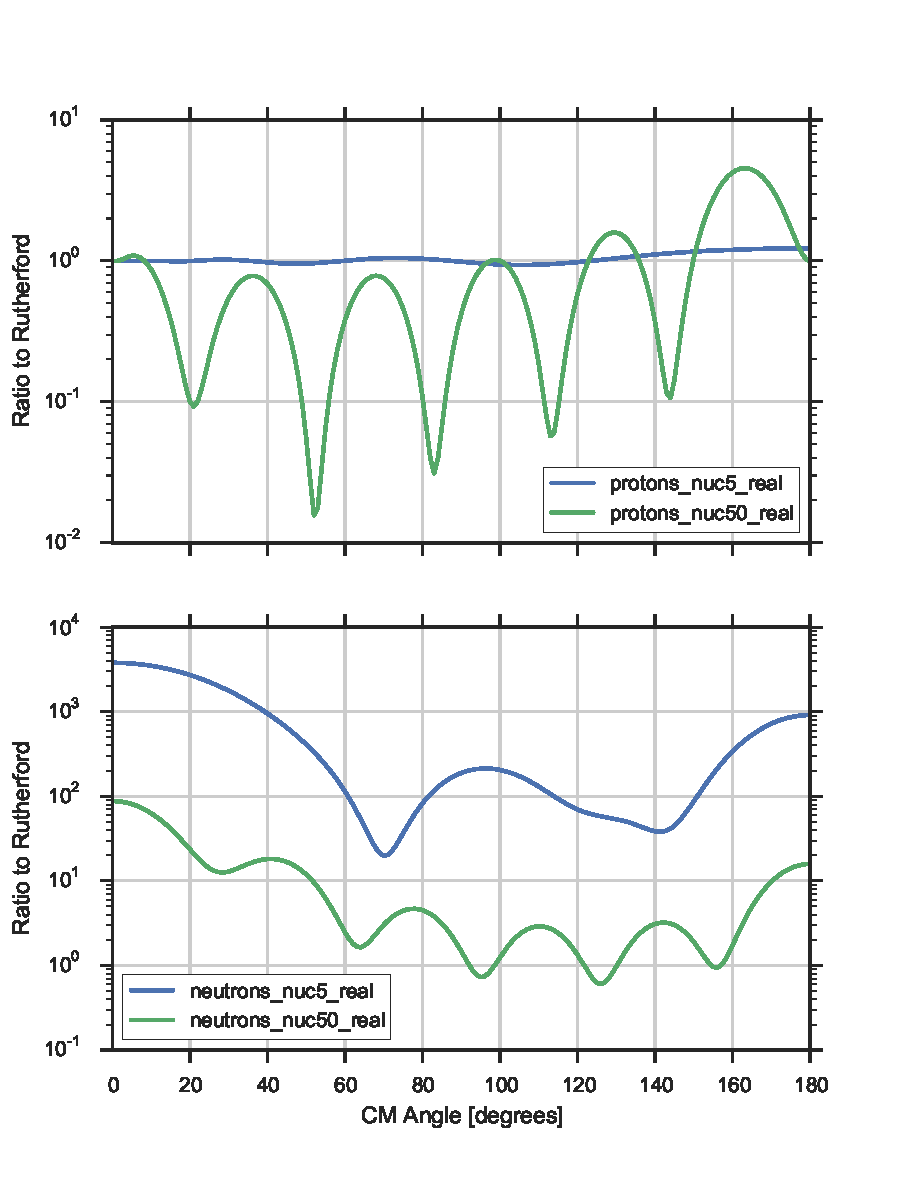
\includegraphics[width=\textwidth]{{images/nuc_real.pdf}}
		\caption{Elastic scattering cross sections on \nuc{100}{Mo} with only the real component of the volume nuclear potential. This is shown for protons (top) and neutrons (bottom) at \SI{5}{MeV} and \SI{50}{MeV}.}
		\label{fig:nuc_real}
	\end{figure}

	\begin{table}
		\centering
		\begin{tabular}{c c c c c c}
			\toprule
			  -0.1406733863 & -0.9900560582  &   0  & 0.5  & 0.5 & : S(L,J,JT) \\
			  -0.9950493561 &  0.0993819851  &   1  & 0.5  & 0.5 & : S(L,J,JT) \\
			  -0.4883262722 &  0.8726611324  &   2  & 1.5  & 1.5 & : S(L,J,JT) \\
			  -0.9950493561 &  0.0993819851  &   1  & 1.5  & 1.5 & : S(L,J,JT) \\
			  -0.4883262722 &  0.8726611324  &   2  & 2.5  & 2.5 & : S(L,J,JT) \\
			\midrule
			  -0.0578241233 & -0.4368748881  &   0 &  0.5 &  0.5  & : S(L,J,JT) \\
			  -0.4404722371 &  0.0377326911  &   1 &  0.5 &  0.5  & : S(L,J,JT) \\
			  -0.2212677416 &  0.3878465564  &   2 &  1.5 &  1.5  & : S(L,J,JT) \\
			  -0.4404722371 &  0.0377326911  &   1 &  1.5 &  1.5  & : S(L,J,JT) \\
			  -0.2212677416 &  0.3878465564  &   2 &  2.5 &  2.5  & : S(L,J,JT) \\
			\bottomrule
		\end{tabular}
		\caption{$S$ matrix elements from \fresco. This is the raw output from the file \texttt{fort.7} for \SI{50}{MeV} protons. The lines above the horizontal rule are for the interaction with only the real part, while the lines below the rule are for the interaction with both real and complex parts. It is clear that the moduli of the upper lines are 1.}
		\label{tab:smat}
	\end{table}

	Then, we tried increasing the radius parameter in the optical potential and the Coulomb potential to \SI{10}{fm}. We found that it greatly increased the number of oscillations in the graph and increased the total cross section. This is what we expected because making the target larger should increase the cross section. The results are shown in Fig.~\ref{fig:big_r}.

	\begin{figure}
		\centering
		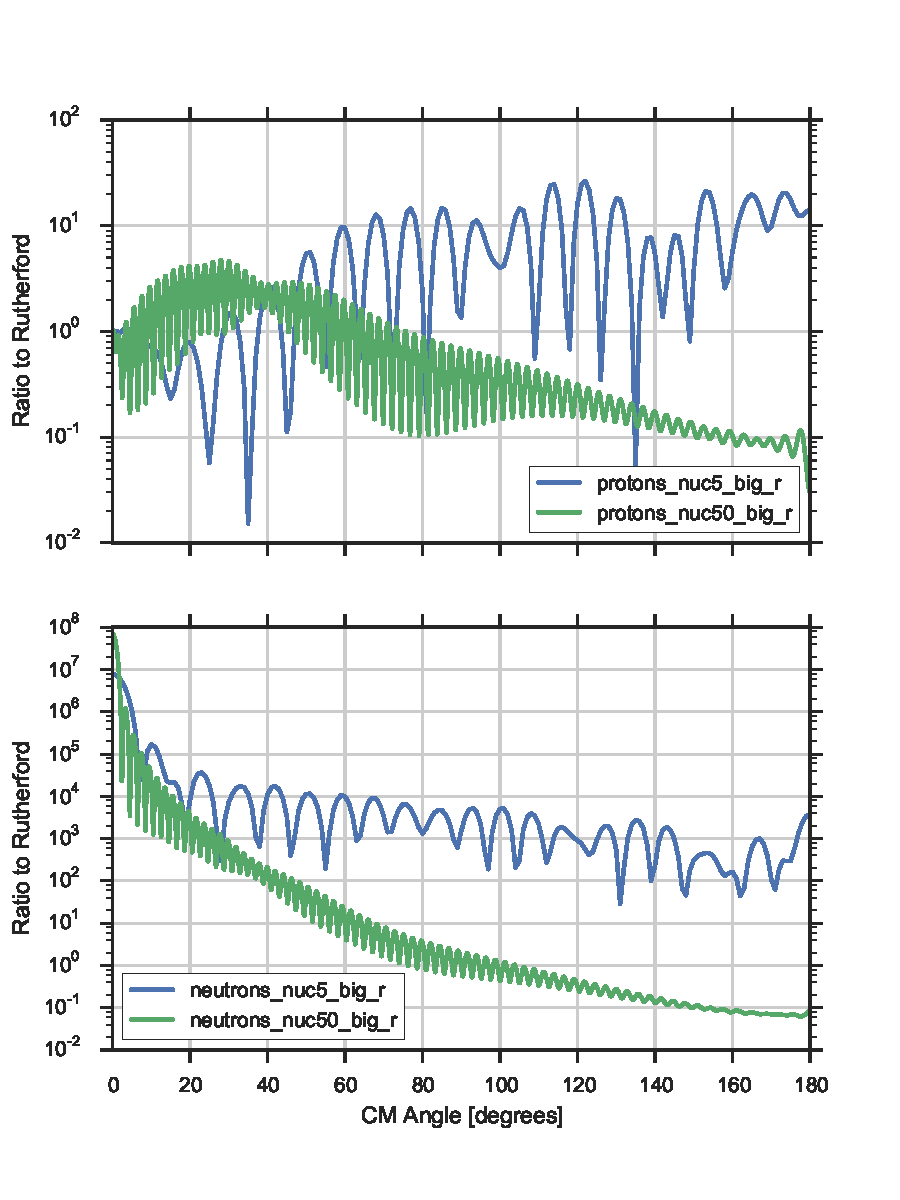
\includegraphics[width=\textwidth]{{images/big_r.pdf}}
		\caption{Elastic scattering with the radius increased to \SI{10}{fm}.}
		\label{fig:big_r}
	\end{figure}

	Finally, we found the total cross sections for neutron elastic scattering at our two energies. These are shown in Table

	\begin{table}
		\centering
		\begin{tabular}{c c c c}
			\toprule
			Energy & Elastic & Absorption & Total \\
			\midrule
			\SI{5}{MeV}  & \SI{4843.87}{mb/sr} & \SI{426.24}{mb/sr} & \SI{5270.11}{mb/sr} \\
			\SI{50}{MeV} & \SI{2597.99}{mb/sr} & \SI{1567.59}{mb/sr} & \SI{4165.57}{mb/sr} \\
			\bottomrule
		\end{tabular}
		\caption{Neutron scattering cross sections from \fresco.}
		\label{tab:xsec}
	\end{table}




\bibliography{hw2}

\end{document}